\subsection{Isolating Loop-Control Offload}
\label{subsec:lcu-loop-control}

We isolated loop-control specialization while retaining the original manually
mapped 4$\times$4 PE mesh and the MMUL and GEM instruction streams. The study
compares the baseline against a 4$\times$4 mesh with one global Loop Control
Unit (LCU), and a 4$\times$5 organization with four row-associated LCUs. The
additional LCUs are control endpoints and do not participate in the toroidal
PE neighbour network. Matrix inputs are identical across configurations at
each size; all output elements match an independent CPU reference for sizes
16, 32, 64, and 128. At size 4, hashes of the dynamic PE operand and state
traces, including memory writes and branch decisions, match across all three
configurations.

Only the three branch operations in each kernel are delegated. MMUL branches
at PCs 8, 16, and 19; GEM branches at PCs 8, 27, and 30. All other PE
instructions, including address updates, remain unchanged. In the modeled
control interface, loop bounds and counters remain in their original PE
registers, the LCU evaluates the branch predicate in parallel with the
existing PC, and a sideband preserves the branch instruction's Rout value.
The four-LCU case broadcasts each predicate to all four units and requires
them to agree on the single global PC target.

\begin{table}[t]
\centering
\caption{Total modeled cycles, including PE program configuration and three
LCU branch entries in the LCU configurations.}
\label{tab:lcu-same-mesh-cycles}
\begin{tabular}{r|rrr|rrr}
\hline
Matrix & \multicolumn{3}{c|}{MMUL} & \multicolumn{3}{c}{GEM} \\
size & OE 4$\times$4 & +1 LCU & +4 LCUs & OE 4$\times$4 & +1 LCU & +4 LCUs \\
\hline
16  & 4,644 & 4,647 & 4,647 & 5,363 & 5,366 & 5,366 \\
32  & 34,584 & 34,587 & 34,587 & 37,319 & 37,322 & 37,322 \\
64  & 268,992 & 268,995 & 268,995 & 279,791 & 279,794 & 279,794 \\
128 & 2,124,048 & 2,124,051 & 2,124,051 & 2,167,103 & 2,167,106 & 2,167,106 \\
\hline
\end{tabular}
\end{table}

The PE execution-cycle count is identical for all configurations at every
size, so execution-only speedup is 1.0. None of the three branch PCs is
control-only: each also issues address or accumulator work on other PEs.
Consequently, moving the branch operation frees a PE instruction slot but
does not remove a global PC or a dynamic execution cycle while preserving the
schedule. The total-cycle figures charge three additional static LCU entries;
the four row LCUs are configured in parallel. Thus, one global LCU and four
LCUs have equal modeled latency, with a fixed three-cycle configuration
overhead relative to the baseline. The corresponding total-cycle speedups are
below 1 by less than 0.07\% at size 16 and approach 1 as the matrix grows.

This result bounds the benefit for the existing schedules: loop control is
not a measurable execution bottleneck once its branch operation overlaps the
same PC. A throughput benefit would require either control-only PCs that can
be removed or a new schedule that uses the released PE slots for useful work.
The LCU operand and Rout sidebands are simulator abstractions; the inspected
RTL does not establish a direct path from arbitrary PE registers into an
LCU. Accordingly, these results demonstrate schedule-level equivalence and
cycle effects under the stated model, not physical LCU timing or a validated
RTL mapping. Figure~\ref{fig:lcu-same-mesh-speedup} summarizes the modeled
speedups.

\begin{figure}[t]
\centering
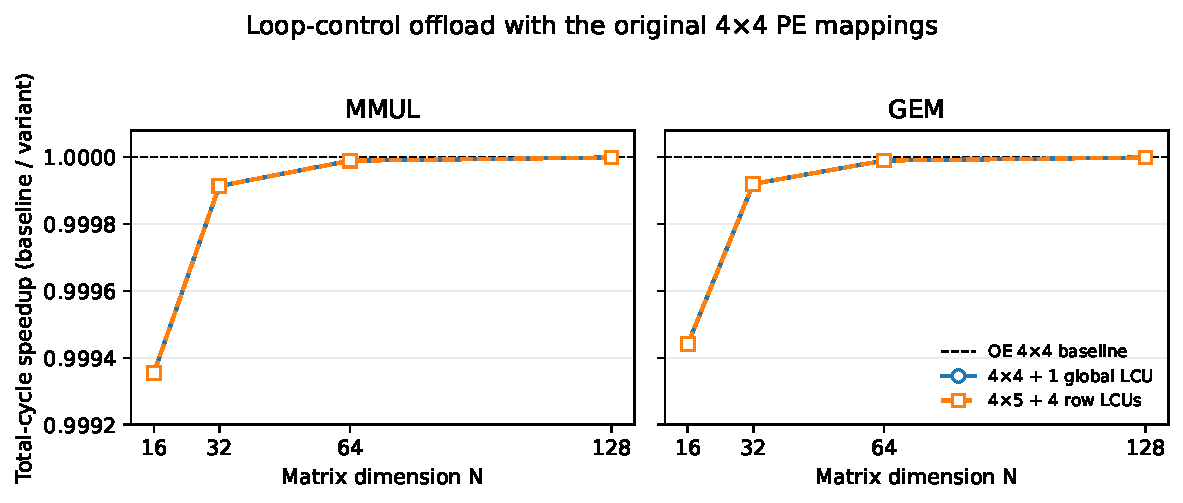
\includegraphics[width=\linewidth]{../benchmarks/DISCOvsOE/heterogeneous/same_mesh_speedup.pdf}
\caption{Total modeled-cycle speedup of the two LCU configurations relative
to the original 4$\times$4 kernels. The vertical axis is zoomed around unity.}
\label{fig:lcu-same-mesh-speedup}
\end{figure}
